\chapter{Vers un Approche de Pronostic Data-Driven}

\begin{chapterintro}
    The goal of this chapter is to introduce the different prognostic approaches with a detailed taxonomy, the various steps of any prognostic approach will be described then the focus will shift towards the data-driven methods.
\end{chapterintro}

\section{Approches Physiques, Data-Driven et Hybrides}

Any prognostics approach is either based on: physical models, data-driven models or a hybrid combination of both of them (Figure \ref{fig:prognostic-approaches-venn}).

\begin{figure}[h]
    \centering
	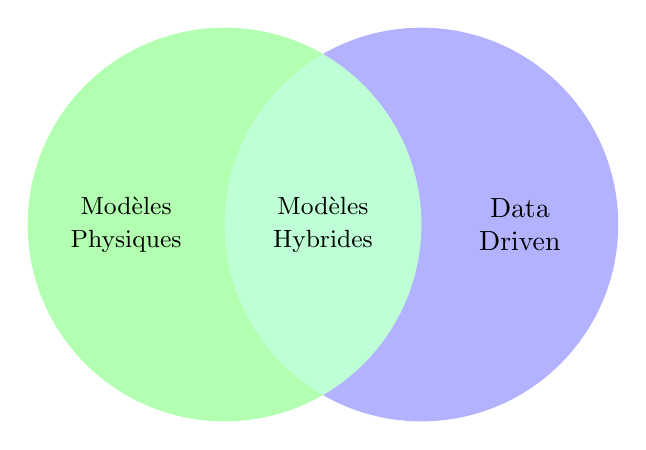
\begin{tikzpicture}
\begin{scope}
[blend group = soft light]
\fill [green!30!white] (0,0) circle (2.5);
\fill [blue!30!white] (2.5,0) circle (2.5);
\end{scope}

\node[text width=2cm, align=center] at (-1.25,0) {\small Modèles Physiques};
\node[text width=1.5cm, align=center] at (3.75,0) { Data Driven};
\node[text width=1.6cm, align=center] at (1.25,0) {\small Modèles Hybrides};
\end{tikzpicture}

    \caption{Taxonomie des approches du pronostic}
    \label{fig:prognostic-approaches-venn}
\end{figure}

These three categories are broad classification based on the followed approach, each one can be further divided into subcategories. A detailed taxonom is presented in Figure \ref{fig:prognostic-approaches-tree}.
\begin{figure}[H]
	\resizebox{\textwidth}{!}{
\begin{tikzpicture}
	[all/.style={draw, minimum height=2em, fill=white, font=\small}]

	\fill [gray!30!white] (-1.41,-6.3) rectangle (1.41,-9.7) ;
	
	\draw(0,0) node[all] (progApp)                       	{Prognostics approaches};
	\draw node[all, below = 1.6em of progApp] (dataDriv)		{Data-Driven};
	\draw node[all, left = 7em of dataDriv] (physBas)      	{Physics-based models};
	\draw node[all, right = 7em of dataDriv] (hybridApp)				{Hybrid models};

	\draw node[all,text width=2cm,align=center,minimum height=3em, below = 1.6em of physBas] (appSpec)		{Application Specific};
	
	\begin{scope}[node distance=1.6em and -3.5em]
		\draw node[all,text width=2cm,align=center,minimum height=3em, below right = of hybridApp] (serApp)		{Series approach};
		\draw node[all,text width=2cm,align=center,minimum height=3em, below left = of hybridApp] (parApp)		{Parallel approach};
	\end{scope}
	
	\begin{scope}[node distance=1.6em and -2.5em]
		\draw node[all,text width=2cm,align=center,minimum height=3em, below right = of dataDriv] (statMod)		{Statistical models};
		\draw node[all,text width=2cm,minimum height=3em, align=center, below left = of dataDriv] (ML)		{Machine Learning};
	\end{scope}

	\begin{scope}[node distance=1.6em and 0em]
		\draw node[xshift=1em,all,text width=2.9cm,align=center,minimum height=3em, below left = of ML] (connect) {Connectionists methods};
		\draw node[all,text width=2.9cm,align=center,minimum height=3em, below = of connect] (instance) {Instance-based learning};
		\draw node[ all,text width=2.9cm,align=center,minimum height=3em, below = of instance] (comb)		{Combined methods};
	\end{scope}

	\begin{scope}[node distance=1.6em and 0em]
		\draw node[xshift=-1em,all,text width=2.9cm,align=center,minimum height=3em, below right = of statMod] (reg)		{Regression methods};
		\draw node[all,text width=2.9cm,align=center,minimum height=3em, below = of reg] (arma)		{ARMA \& variants};
		\draw node[all,text width=2.9cm,align=center,minimum height=3em, below = of arma] (propor)		{Proportional hazard methods};
	\end{scope}

	\begin{scope}[node distance=1.6em and 0em]
	\path let \p1 = (connect) in node[all,text width=2.3cm,align=center,minimum height=3em] (bayes)	at (0,\y1)	{Bayesian methods};
	\draw node[all,text width=2.3cm,align=center,minimum height=3em, below  = of bayes] (hmm)		{Markov models};
	\draw node[all,text width=2.3cm,align=center,minimum height=3em, below  = of hmm] (sotch)		{Stochastic filtering};
	\end{scope}

	\draw[->, >=angle 60] (progApp.south)   -- ++(0,0) -- ++(0,-0.8em) -| (physBas.north);
	\draw[->, >=angle 60] (progApp.south)   -- ++(0,0) -- ++(0,-0.8em) -| (hybridApp.north);
	\draw[->, >=angle 60] (progApp.south)   --  (dataDriv.north);
	
	\draw[->, >=angle 60] (physBas.south)   --  (appSpec.north);
	
	\draw[->, >=angle 60] (hybridApp.south)   -- ++(0,0) -- ++(0,-0.8em) -| (parApp.north);
	\draw[->, >=angle 60] (hybridApp.south)   -- ++(0,0) -- ++(0,-0.8em) -| (serApp.north);
	
	\draw[->, >=angle 60] (dataDriv.south)   -- ++(0,0) -- ++(0,-0.8em) -| (statMod.north);
	\draw[->, >=angle 60] (dataDriv.south)   -- ++(0,0) -- ++(0,-0.8em) -| (ML.north);
	
	\draw[->, >=angle 60] ([xshift=-1em]ML.south)   |- (connect.east);
	\draw[->, >=angle 60] ([xshift=-1em]ML.south)   |- (instance.east);
	\draw[->, >=angle 60] ([xshift=-1em]ML.south)   |- (comb.east);
	
	\draw[->, >=angle 60] ([xshift=1em]statMod.south)   |- (reg.west);
	\draw[->, >=angle 60] ([xshift=1em]statMod.south)   |- (arma.west);
	\draw[->, >=angle 60] ([xshift=1em]statMod.south)   |- (propor.west);

	\draw[->, >=angle 60] (ML.south)   -- ++(0,0) -- ++(0,-0.8em) -| (bayes.north);
	\draw[-] (statMod.south)   -- ++(0,0) -- ++(0,-0.8em) -| (bayes.north);
	\draw[->, >=angle 60] (bayes.south)   -- (hmm.north);
\end{tikzpicture}
}
    \caption{Taxonomie des approches du pronostic}
    \label{fig:prognostic-approaches-tree}
\end{figure}



%\begin{figure}[h]
 %   \centering
  %  \begin{tikzpicture}
 \pie [polar]
    {56/Statistique,
     26/Machine Learning, 10/Physique,8/Hybride}
\end{tikzpicture}
 %   \caption{}
  %  \label{fig:prognostic-approaches-literature-statistics}
%\end{figure}


\subsection{Modèles Physiques}
Physical models assess the health of the system using explicit mathematical formulation (white boxes) developed based on scientific and engineering understanding of its behavior. However, the main advantage of these physical models consists of using degradation models to predict long-term behaviour \cite{Cubillo2016}.

The physics model-based approaches are able to provide accurate estimation of RUL if the physics model is developed with complete understanding of the failure mechanisms and effective estimation of model parameters. For some complex mechanical systems, however, it is difficult to understand the physics of damage, which restricts the application of these approaches \cite{Lei2018}.

\subsection{Modèles Data-Driven}
Data-Driven models rely on previously collected data (monitoring data, operational settings data, …) to establish a model able to assess the health of the system and predict its behaviour and degradation.
In contrast to physical models, and as the name implies, data-driven models don't rely on human knowledge but mainly on collected historic data to model the degradation process. Usually data-driven models are considered as black boxes.

\subsubsection{Modèles Statistiques}
Statistical approach, for the estimation of RUL, relies on constructing and fitting a probabilistic model to the past obeserved data without relying on any physical or engineering principles \cite{Si2011}. 
% TODO: finish this shit
The authors of \cite{Si2011} presented a review on statistical data-driven approaches for prognostics, according to this review, many models fall into this category such as regression models (e.g. linear regression), autoregressive-moving average and its variants, stochastic filtering techniques (Kalman Filter, Particles Filter, …).

\subsubsection{Machine Learning}
Machine learning is a field of Artificial Intelligence that exploded in the recent years and made breakthroughs in many fields such as computer vision and nautral language processing. Machine learning models are black-box models that can discover even very complex mapping from an input to an output. Many types of models fall into this category like connectionist methods (e.g. Artificial Neural Networks), Instance-Based Learning (e.g. Support-Vector Machines). Different approaches can be combined together to create combined machine learning models that can perform better than a single model.

\subsection{Modèles Hybrides}
Hybrid models are a combination of a physical-based model and a data-driven one.
There are two types of hybrid models depending on how the physical and data-driven models are combined.
The data-driven can be integrated within a physical model in serial configuration (Figure \ref{fig:hybrid-approach-series}) where it is used to tune the parameters of the physical model which then makes predicitons.

\begin{figure}[h]
    \centering
    \begin{tikzpicture}
 	\node[draw, rectangle] (ph) {Physics based approach};
 	\node[draw, rectangle, below = 3em of ph] (dd) {Data-driven approach};
 	
 	\draw[->, >=angle 60] (dd.north) -- node[right] {\scriptsize  Parameter tuning} (ph.south);
 	\draw[->, >=angle 60] (ph.east) -- node[above] {\scriptsize Prediction} ([xshift=4.5em]ph.east);
 	\draw[->, >=angle 60] (-4.5,0) -- node[above] {\scriptsize Input} (ph.west);
	\draw[->, >=angle 60] (-3,0) |-  (dd.west);
\end{tikzpicture}
    \caption{Configuration hybride en série (Figure adaptée de la référence \cite{Mangili2013})}
    \label{fig:hybrid-approach-series}
\end{figure}

Both of data-driven and physical models can be combined in parallel configuration (Figure \ref{fig:hybrid-approach-parallel}) where both of the models make seperate predicitons which can be combined to come up with the final estimation.
\begin{figure}[h]
    \centering
    \begin{tikzpicture}
    \node[draw, rectangle] (ph) {Physics based approach};
    \node[draw, circle, below = 1em of ph] (u) {U};
    \node[draw, rectangle, below = 1em of u] (dd) {Data-driven approach};

    \draw[->, >=angle 60] (u.east)      --      node[above] {\scriptsize Prediction} ([xshift=4.5em]u.east);
    \draw[->, >=angle 60] (ph.south)    --      (u.north);
    \draw[->, >=angle 60] (dd.north)    --      (u.south);
    \draw[->, >=angle 60] (-4.5,0)      --      node[above] {\scriptsize Input} (ph.west);
    \draw[->, >=angle 60] (-3,0)        |-      (dd.west);
    %the following lign is just to make the figure center precisely and align with the previous one
    \draw[->, draw=none] (ph.east) -- ([xshift=4.5em]ph.east);
\end{tikzpicture}
    \caption{Configuration hybride parallèle (Figure adaptée de la référence \cite{Mangili2013})}
    \label{fig:hybrid-approach-parallel}
\end{figure}

\section{Pourquoi un Approche Data-Driven?}


\section{Conclusion}
% TODO: finish this shit too
The classification of various prognostic approaches was introduced and divided into three main categories: 1) Physical models, 2) Data-Driven models and 3) Hybrid models. Detailed taxonomy was presented and the different examples were given. The focus now will shift toward data-driven models.